\documentclass[journal,twoside,web]{ieeecolor}
\usepackage{generic}
\usepackage{cite}
\usepackage{amsmath,amssymb,amsfonts}
\usepackage{graphicx}
\usepackage{booktabs}
\usepackage{array}
\usepackage{multirow}
\usepackage{textcomp}
\usepackage{url}

\newcommand{\zonecap}{ZoneCap}
\newcommand{\Adm}{\operatorname{Adm}}
\newcommand{\Emit}{\operatorname{Emit}}
\newcommand{\Tr}{\operatorname{Tr}}
\newcommand{\Reach}{\operatorname{Reach}}
\newcommand{\NA}{\textnormal{N/A}}

% Target-hardware study (exp-22--25). Set to true only after the returned
% directories pass the research audit and the human accepts the S3 review;
% then run figures/build_c5_results.py, which writes the numbers and the
% mechanically selected outcome case used by every conditional passage.
\newif\ifzonecaphardware
\zonecaphardwarefalse
\newcommand{\cfive}[1]{\ifcsname cfive@#1\endcsname\csname cfive@#1\endcsname\else\textbf{??#1}\fi}
\ifzonecaphardware
\input{figures/generated/c5_numbers}
\fi

\markboth{IEEE Transactions on Industrial Informatics, under review}{}

\begin{document}

\title{ZoneCap: Attenuable Capabilities Linking Industrial Zone/Conduit Policy to Physical Reachability}
\author{Anonymous~Authors}

\maketitle

\begin{abstract}
Industrial control commands increasingly cross zone and organizational boundaries through delegated software principals. Capability attenuation can narrow digital permissions, while cyber-physical runtime enforcers can suppress or correct commands, but neither property alone orders the physical behavior induced by parent and child authority. We present ZoneCap, a source-table compiler and runtime authorization semantics that bind zone/conduit topology to attenuable caveats over assets, actions, physical parameters, time, operating mode, and required event history. Under six explicit obligations, positive conjunctive attenuation yields request-abstracted emission inclusion and, consequently, finite-horizon physical trace and reachable-set inclusion. An exact audit covered 393,750 one-dimensional models and 2,756,250 horizon checks without an inclusion violation, while premise-removal tests recovered the expected counterexamples. On a frozen 58,968-case corpus derived from a CPwE/CIP Security zone/conduit matrix, an ENISA landside-signalling subgraph, and a declared evaluation overlay, the compiler matched a separate table oracle on every decision and passed 672 delegation-dimension checks. The registered five-effect actuation-event semantics produced no safety or refinement violation over 58,968 one-request traces, 4,536 composed traces, and 492,156 exhaustively enumerated words. Fair delayed revocation delivery nevertheless exposed eight issuance-relative stale executions. Target OpenPLC/Jetson performance was not measured, and no performance claim is made. ZoneCap therefore provides a bounded, inspectable authorization-to-physics refinement contract, not a guarantee under mismatched plant models, compromised context, fixed-tick execution, or unspecified revocation freshness.


\end{abstract}

\begin{IEEEkeywords}
Authorization, capability-based security, cyber-physical systems, industrial control systems, runtime enforcement.
\end{IEEEkeywords}

\section{Introduction}
\label{sec:introduction}

\IEEEPARstart{I}{ndustrial} control commands increasingly cross organizational and network boundaries before they reach a physical process. Maintenance services, supervisory applications, and autonomous software principals may receive authority to inspect or actuate assets in another security zone~\cite{iec62443}. Network segmentation constrains where communication can flow, but delegated actuation also depends on the target asset, operation, physical parameter, time, operating mode, and preceding events. A runtime authorization object must preserve these restrictions as authority moves between principals. More importantly, an industrial operator needs to know whether narrowing that object also narrows the physical behavior the delegate can induce.

Capability systems offer a natural basis for delegated least privilege. Cyber-physical capability architectures combine local architectural protection with cryptographic tokens~\cite{dodson2021,dodson2020}, and recent agent-facing systems add signed physical constraints, attenuation, revocation, approvals, and audit~\cite{sint2026,ranathunga2026,bamil2026}. Their digital ordering does not, by itself, order plant behavior. A child may submit different requests from its parent, and an enforcement layer may replace, delay, or suppress those requests. Syntactic scope inclusion must therefore be connected to the set of physical inputs actually emitted at runtime.

Physics-aware access control and runtime enforcement address the downstream problem from complementary directions. Model-informed policies can reject actions whose predicted consequences violate a physical condition~\cite{etigowni2016,rafy2026}. Edit-automata and industrial I/O enforcers can suppress or correct compromised-controller events, with established soundness, progress, and scalability properties~\cite{ligatti2005,pearce2020,lanotte2023,baird2024}. Separately, IEC~62443-3-2 structures industrial risk assessment around zones and conduits~\cite{iec62443}. These lines do not specify a common refinement relation from zone/conduit-derived delegation syntax, through a command-editing enforcement point, to the physical traces admitted by the plant.

This paper introduces \zonecap{}, which makes that missing interface explicit. A source-table compiler converts directed zone/conduit grants and declared physical caveats into capabilities, while a field-wise validator restricts every delegated child. At runtime, five authorization effects map requests to checked physical emissions, registered holds, or no actuation event. The central insight is a three-step refinement: positive conjunctive attenuation establishes authorization inclusion; sound and parent-realizable effects establish request-abstracted emission inclusion; and a common plant relation lifts emission inclusion to finite-horizon trace and reachable-set inclusion. Fig.~\ref{fig:overview} summarizes the path.

\begin{figure*}[t]
\centering
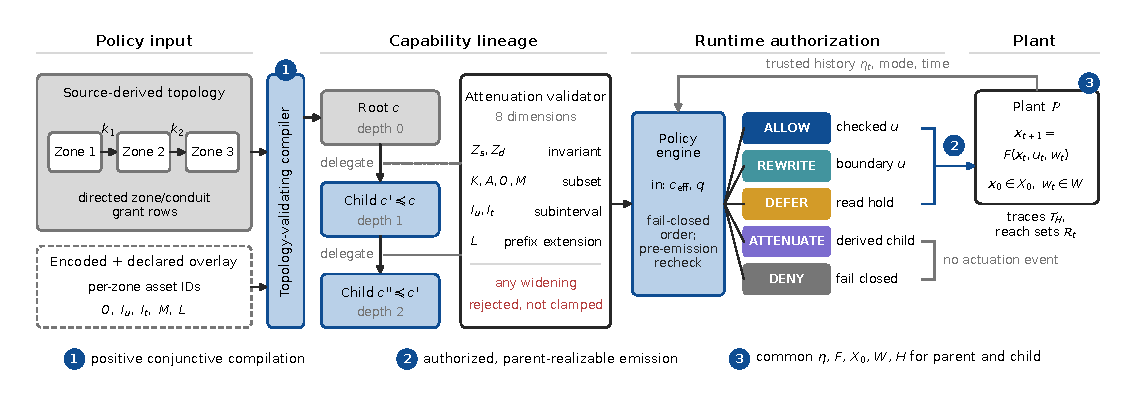
\includegraphics[width=\textwidth]{figures/generated/fig01_zonecap_overview}
\caption{ZoneCap compilation, delegation, enforcement, and physical-refinement path. The grey block is the source-derived zone/conduit topology; the dashed block holds per-zone asset identifiers and the declared evaluation overlay, which the sources do not supply. The validator checks eight authority dimensions without querying plant reachability. \texttt{DENY} and \texttt{ATTENUATE} emit no actuation event; the figure depicts actuation-event semantics, not fixed-tick PLC execution. Numbered badges mark the interfaces at which Section~\ref{sec:theorem} imposes obligations: (1)~positive conjunctive compilation, (2)~authorized and parent-realizable emission, and (3)~a common history projection, plant relation, uncertainty set, and horizon for parent and child.}
\label{fig:overview}
\end{figure*}


The paper makes the following contributions:
\begin{itemize}
    \item It establishes a conditional refinement theorem from field-wise capability attenuation to physical trace and reachable-set inclusion. Six explicit obligations separate the result from same-request behavior, controller synthesis, and model-mismatch robustness.
    \item It develops a zone/conduit-table compiler and validates it on frozen CPwE/CIP Security and ENISA landside-signalling inputs augmented by a declared source-independent overlay. Complete-corpus, mutation, provenance, path, and delegation checks test the concrete realization.
    \item It defines an actuation-event semantics for \texttt{ALLOW}, \texttt{DENY}, \texttt{ATTENUATE}, \texttt{REWRITE}, and \texttt{DEFER}, and evaluates refinement, composition, effect coverage, and deny-only service loss in the registered bounded model.
\end{itemize}
The evaluation also reports a negative result: fair delayed revocation delivery admits issuance-relative stale execution even when resolver-local post-delivery invariants remain intact. This boundary shows that physical refinement and lifecycle safety require explicit operational contracts rather than an unqualified claim of safe attenuation.

\section{Related Work and Design Gap}
\label{sec:related}

\subsection{Capabilities and Delegated Authorization}

Capability systems bind authority to explicit objects and support delegation without relying on ambient principal privileges. Dodson's cyber-physical capability architecture and CHERI Macaroons combine architectural capabilities with cryptographic network tokens, allowing scoped authority to be constructed, delegated, and exercised in robotics and industrial-control demonstrators~\cite{dodson2021,dodson2020}. SINT extends this direction to agent-facing gateways through signed tokens, physical maxima, attenuation-only delegation, revocation, approval tiers, and audit logging~\cite{sint2026}. ZTPM represents physical impact and live context as typed runtime policy dimensions for agents that control robots~\cite{ranathunga2026}, whereas DARC expresses multi-agent handoffs as contracts with attenuation, obligations, lineage, and revocation closure~\cite{bamil2026}. These systems establish practical and formal foundations for delegated physical authority. They do not establish when field-wise attenuation remains a refinement after a runtime layer rewrites or defers commands and a plant evolves.

\subsection{Physics-Aware Authorization and Runtime Enforcement}

Physics-aware authorization and runtime enforcement constrain commands through different mechanisms. CPAC derives access-control decisions from information flow over a physical grid model~\cite{etigowni2016}, and TwinGridShield evaluates grid-agent actions against a deterministic network twin while exposing sensitivity to model mismatch~\cite{rafy2026}. Runtime enforcement instead mediates an event stream: security automata characterize suppressible policies~\cite{schneider2000}, edit automata add insertion and replacement~\cite{ligatti2005}, Smart I/O places mediation close to industrial I/O~\cite{pearce2020}, and Lanotte \emph{et al.} synthesize monitors that correct or suppress compromised-controller actions with soundness and progress guarantees~\cite{lanotte2023}. Baird \emph{et al.} address scalable composition of such policies~\cite{baird2024}. \zonecap{} does not replace these mechanisms or claim greater enforcement throughput. It specifies the delegated authorization relation and the output contract an enforcer must satisfy for the child's induced physical behavior to remain within the parent's.

\subsection{Industrial Zone/Conduit Modeling}

IEC~62443-3-2 uses zones and conduits as central abstractions in security-risk assessment for industrial automation and control systems~\cite{iec62443}. Recent work automates parts of that risk-assessment workflow from engineering and threat models~\cite{dasilva2025}, and an IEC~62443-oriented domain-specific language formalizes zone/conduit installations and validation rules~\cite{vaudey2024}. These contributions operate primarily at design time; they do not turn a directed zone/conduit grant into a delegatable runtime object with an associated physical refinement relation. \zonecap{} uses selected, published zone/conduit structures as frozen compiler inputs, augments them with an explicitly declared evaluation overlay, and connects the resulting capabilities to runtime emissions and plant reachability. Only the zone/conduit topology is source-derived; target assets are deterministic encodings, and the behavioral and contextual fields are a declared overlay. This use is neither an implementation of the complete standard nor evidence of IEC~62443 conformance or certification.


\section{System Model and Problem Statement}
\label{sec:model}

\subsection{System and Trust Model}

We consider cross-zone actuation in which a policy authority issues a capability to a software principal, the principal may delegate a narrower child capability, and a policy enforcement point mediates requests before they reach the plant. The trusted computing base comprises the source-table compiler, capability issuer, attenuation validator, effect binding, and providers of authorization-relevant time, mode, and plant history. The network and requesting principal need not be trusted. The refinement result assumes that parent and child executions use the same history projection and plant transition relation; compromised sensors, stale modes, and model mismatch are outside that result.

Let the plant be the discrete-time transition system
\begin{equation}
    \mathcal{P}=(X,U,W,F), \qquad x_{t+1}=F(x_t,u_t,w_t),
    \label{eq:plant}
\end{equation}
where $X_0\subseteq X$ is the initial-state set, $U$ is the set of physical inputs, and $W$ is a fixed disturbance set. An authorization-relevant physical history $\eta_t$ records observed plant states, emitted physical events, trusted operating mode, and time. It excludes token-internal decisions and raw requests that produced no actuation event.

\subsection{Capability and Attenuation}

A \zonecap{} capability is the tuple
\begin{equation}
 c=(\mathit{iss},\mathit{sub},Z_s,Z_d,K,A,O,I_u,I_t,M,L),
 \label{eq:capability}
\end{equation}
which binds an issuer and subject to source and destination zones, conduit set $K$, asset set $A$, operation set $O$, parameter interval $I_u$, time window $I_t$, operating-mode set $M$, and admissible physical-history language $L$. Compilation maps $c$ and history $\eta$ to an authorization relation $\Adm_c(\eta)\subseteq U$. Table~\ref{tab:fields} records the source and attenuation treatment of each authority field.

\begin{table*}[t]
\caption{ZoneCap capability fields, provenance, and attenuation rules. Structural source fields are separated from the declared evaluation overlay.}
\label{tab:fields}
\centering
\footnotesize
\setlength{\tabcolsep}{4pt}
\begin{tabular}{@{}llll@{}}
\toprule
Field & Meaning & Evaluation provenance & Child rule/runtime check \\
\midrule
$Z_s,Z_d$ & Zone endpoints & Source-derived topology & Invariant; exact endpoint match \\
$K$ & Directed conduits & Source-derived topology & Set subset; valid endpoint path \\
$A$ & Target assets & Deterministic per-zone encoding & Set subset; requested asset membership \\
$O$ & Operations & Source-independent overlay & Set subset; requested operation membership \\
$I_u$ & Physical parameter envelope & Source-independent overlay & Interval subset; value or rewrite membership \\
$I_t$ & Validity window & Source-independent overlay & Interval subset; trusted time membership \\
$M$ & Operating modes & Source-independent overlay & Set subset; trusted mode membership \\
$L$ & Required event histories & Source-independent overlay & Language refinement; sequence-prefix check \\
\bottomrule
\end{tabular}
\end{table*}

A child $c'\preceq c$ preserves the issuer and zone endpoints while narrowing every authority dimension:
\begin{equation}
\begin{split}
K'&\subseteq K,\; A'\subseteq A,\; O'\subseteq O,\; I'_u\subseteq I_u,\\
I'_t&\subseteq I_t,\; M'\subseteq M,\; L'\subseteq L.
\end{split}
\label{eq:attenuation}
\end{equation}
The subject may change because delegation transfers identity while narrowing physical authority. The implementation represents $L$ by an ordered required-event sequence and requires the parent's sequence to be a prefix of the child's. This rule is sufficient for history-language inclusion. Relation~\eqref{eq:attenuation} contains neither plant dynamics nor a reachable-set predicate, so the desired result is not true by definition.

\subsection{Request-Abstracted Physical Behavior}

For raw request $q\in Q$, $\Emit_c(\eta,q)\subseteq U$ denotes the physical input emitted by the runtime effect. Reachability uses the request-abstracted relation
\begin{equation}
    \overline{E}_c(\eta)=\bigcup_{q\in Q}\Emit_c(\eta,q).
    \label{eq:emission}
\end{equation}
This union does not require same-request output inclusion. For example, a parent with interval $[0,1]$ may allow request $0.8$, whereas a child with interval $[0,0.4]$ rewrites the same request to $0.4$. The child output remains realizable under the parent even though the two same-request outputs differ.

Let $\Tr_H(c)$ contain all physical traces of length at most $H$ from $X_0$, with $w_t\in W$ and $u_t\in\overline{E}_c(\eta_t)$. We define
\begin{equation}
 \Reach_t(c)=\{x_t\mid(x_0,u_0,w_0,\ldots,x_t)\in\Tr_H(c)\}.
 \label{eq:reach}
\end{equation}
The research question is whether the syntactic relation $c'\preceq c$ implies inclusion of these physical traces and reachable sets after runtime mediation. This question excludes probability ordering, a selected controller trajectory, controller synthesis, and universal robustness to an incorrect plant or context model.


\section{ZoneCap Design}
\label{sec:design}

\zonecap{} connects five interfaces: source-table normalization, capability compilation, attenuation validation, runtime decision, and physical effect binding. The first two convert a directed zone/conduit grant into a root capability. Delegation applies field-wise subset checks, after which the policy engine selects an effect and the binding either emits an authorized physical input, emits the registered hold, or emits no actuation event. Fig.~\ref{fig:overview} identifies the obligations exposed at each interface.

\subsection{Source-Table Compilation}

The compiler accepts named zones, directed conduits, and grant rows. It rejects duplicate or unknown identifiers, mismatched conduit endpoints, assets or operations outside a row's scope, and parameter intervals outside the conduit envelope. A valid row becomes a root capability whose issuer and zone endpoints remain invariant under delegation. Other fields are positive caveats combined by intersection, which prevents a narrower caveat from activating a fallback grant and provides the monotone structure used by Lemma~1 in Section~\ref{sec:theorem}.

The evaluation sources do not supply every field in~\eqref{eq:capability}. The CPwE/CIP Security matrix and the ENISA landside-signalling subgraph provide the directed zone/conduit topology~\cite{cpwe2020,enisa2022}. During encoding, each target zone receives a deterministic target-asset identifier. A common source-independent overlay supplies read/write operations, normalized parameter and time intervals, operating modes, and an authenticate pre-action sequence. Provenance metadata keeps these encoded and overlaid fields separate; the compiler therefore tests a bounded zone/conduit realization rather than claiming that the sources or IEC~62443 define the complete capability.

\subsection{Attenuation Validation}

Given a proposed child, the validator checks issuer equality, invariant zone binding, set inclusion for conduits, assets, operations, and modes, interval inclusion for parameters and time, and prefix extension for the required sequence. It rejects an invalid child instead of silently normalizing it. A valid delegation may replace the subject and increments the recorded depth, but it preserves lineage and cannot widen any of the eight checked authority dimensions. The validator never queries plant reachability, so syntactic attenuation remains independently falsifiable.

\subsection{Runtime Decision and Effect Binding}

The policy engine evaluates a request in a fixed, fail-closed order. Missing context or a registered high-risk condition returns \texttt{DEFER}. A failed subject, zone, conduit, asset, operation, time, mode, or history check returns \texttt{DENY}. A runtime parameter envelope that strictly narrows the presented interval returns \texttt{ATTENUATE} with a derived child capability and does not execute the request. A structurally valid value outside the effective interval returns \texttt{REWRITE} to the nearest authorized boundary. A request that passes all checks returns \texttt{ALLOW}.

The physical binding gives each decision an actuation-event meaning. \texttt{ALLOW} emits the checked request, and \texttt{REWRITE} emits only the checked boundary value. \texttt{DEFER} emits the registered read hold only when it is authorized and parent-realizable. \texttt{DENY} and \texttt{ATTENUATE} emit no actuation event. A bounded resolver tracks consecutive deferrals and returns a no-output denial after the resolution limit; an invalid rewrite or hold also fails closed. These rules do not describe fixed-tick PLC execution, where the plant may evolve between commands and a common idle binding would need separate verification.

\subsection{Enforcement and Revocation Interface}

Immediately before emission, the enforcement point repeats effective-capability membership and records the decision, emitted value, lineage, context version, and revocation state for audit. Revocation delivery is a resolver-local transition that marks a holder revoked and removes its pending command. Revocation issuance at a remote authority service is a distinct event. The local interface makes no implicit claim that issuance and delivery are atomic; Section~\ref{sec:discussion} evaluates the consequence of that distinction.


\section{Physical Refinement Guarantee}
\label{sec:theorem}

The same-request example in Section~\ref{sec:model} shows why field-wise attenuation alone does not order runtime outputs. \zonecap{} instead separates authorization inclusion from emission inclusion and requires parent realizability at their interface. Fig.~\ref{fig:refinement} summarizes this proof chain and instantiates the resulting reachable-set relation on three exact signed one-dimensional plants.

\begin{figure*}[t]
\centering
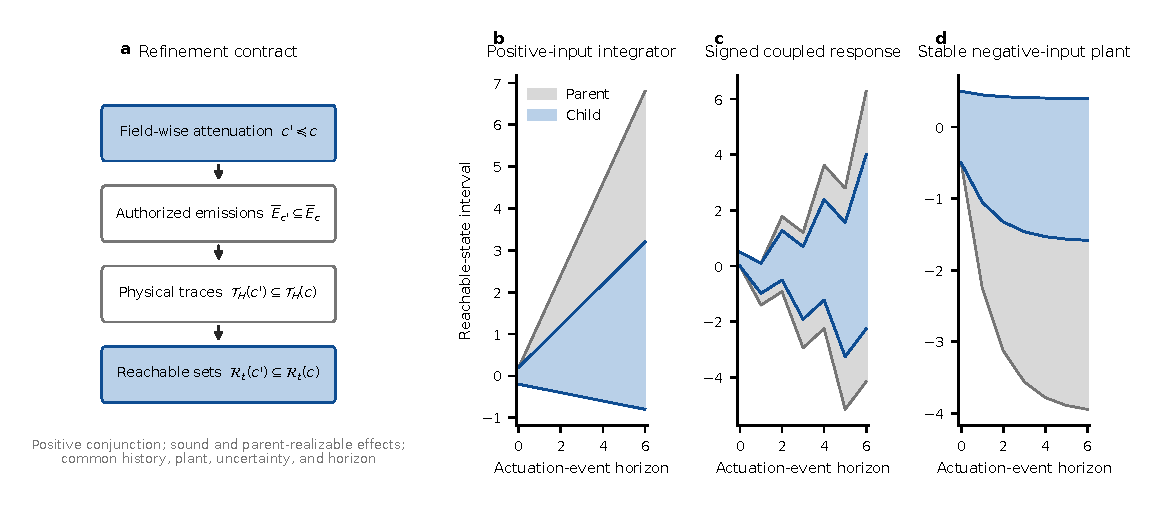
\includegraphics[width=\textwidth]{figures/generated/fig02_refinement_reachability}
\caption{Attenuation-to-reachability refinement and exact instantiations. (a) The proof factors field-wise attenuation through request-abstracted emission and physical-trace inclusion. (b)--(d) Parent and child reachable intervals through actuation-event horizon six for a positive-input integrator, a signed coupled response, and a stable negative-input plant. Grey denotes the parent domain and blue the child domain. The intervals were propagated with seedless exact rational arithmetic; no sampling error bars apply. These panels check executable instances, whereas Theorem~1 establishes the conditional general result.}
\label{fig:refinement}
\end{figure*}

\subsection{Proof Obligations}

The refinement requires six obligations. First, attenuation is the syntactic order in~\eqref{eq:attenuation}, not a definition based on emissions or reachability. Second, positive caveats combine conjunctively; fallback grants and unproved non-monotone conflict combiners are excluded. Third, the child history language refines the parent's, and both evaluate the same physical-history projection. These obligations constrain capability construction.

Three further obligations connect authorization to the plant. Fourth, every emitted rewrite or hold is within the effective capability and parent-realizable; no-command effects contribute no actuation event. Fifth, parent and child use identical $F$, $X_0$, $W$, and horizon. Sixth, reachability is the union over all admitted physical-input and disturbance sequences. It is not a same-request noninterference property, a probability distribution, or a selected controller trajectory.

\subsection{Compiler and Emission Refinement}

\noindent\textbf{Lemma 1 (compiler refinement):} Under obligations 1--3,
\begin{equation}
 c'\preceq c \Longrightarrow
 \Adm_{c'}(\eta)\subseteq\Adm_c(\eta), \quad \forall\eta.
 \label{eq:compiler-refinement}
\end{equation}
Every primitive child domain is a subset of its parent domain. Membership in their positive conjunction therefore implies membership in the parent conjunction. Extending the required event sequence also makes every child-accepted physical history parent-accepted. This argument uses no semantic reachability premise.

\noindent\textbf{Lemma 2 (emission refinement):} Under Lemma~1 and obligation~4,
\begin{equation}
 \overline{E}_{c'}(\eta)\subseteq\overline{E}_c(\eta), \quad \forall\eta.
 \label{eq:emission-refinement}
\end{equation}
Soundness places each ordinary child output in $\Adm_{c'}(\eta)$ and hence in $\Adm_c(\eta)$. Parent realizability supplies a raw parent request that emits the same action. The common hold clause covers a deferred child, while no-output effects add no action to~\eqref{eq:emission}. Authorization membership alone would be insufficient because a parent enforcer could be sound yet unable to produce the child's chosen correction.

\subsection{Trace and Reachable-Set Inclusion}

\noindent\textbf{Theorem 1 (attenuation monotonicity):} Under obligations 1--6, for every finite $H$,
\begin{equation}
 \begin{split}
 c'\preceq c &\Longrightarrow \Tr_H(c')\subseteq\Tr_H(c),\\
 \Tr_H(c')\subseteq\Tr_H(c) &\Longrightarrow
 \Reach_t(c')\subseteq\Reach_t(c),\quad t\leq H.
 \end{split}
 \label{eq:main-theorem}
\end{equation}
The proof is induction on physical transitions. Length-zero traces share $X_0$. Suppose a child trace through $\eta_t$ is also a parent trace. Lemma~2 places its next input in the parent emission relation at the same history. Choosing the same $w_t\in W$ and applying the common $F$ produces the same successor. The extended child trace is therefore a parent trace, and projection onto $x_t$ yields reachable-set inclusion.

For $x_{t+1}=a x_t+b u_t+w_t$ with interval sets, linear images and Minkowski addition preserve inclusion for signed $a$ and $b$, giving an exact one-dimensional corollary. The transition-system proof also covers MIMO and nonlinear plants whenever~\eqref{eq:emission-refinement} holds at every related history. A convex over-approximation alone does not establish this relation. Non-monotone grants, an unauthorized or parent-unrealizable effect, mismatched history or plant semantics, and an unverified fixed-tick idle action are explicit failure conditions rather than implementation details.

\section{Evaluation Methodology}
\label{sec:evaluation}

The evaluation asked whether the implementation preserved the formal refinement, compiled the frozen zone/conduit inputs correctly, and composed all five runtime effects without violating the registered semantics. The protocol was fixed before confirmatory execution. Development fixtures were excluded, exact runs were seedless, and the MIMO/history study reported all five preregistered seeds. Every run retained its configuration, command, log, metrics, and input/output hashes. Perfect agreement triggered predefined dependency, mutation, provenance, and disabled-check audits.

The theorem was evaluated through a proof and falsification ladder rather than statistical confirmation. Exact rational arithmetic covered the registered one-dimensional grid. Additional runs mutated each caveat and combiner, tested coupled MIMO and history-dependent plants, removed and restored rewrite/hold premises, exercised a fair common capability subset, and checked fixed boundary cases. Randomized plants tested registered alternatives but were not treated as evidence for the theorem's universality.

Compiler evaluation used the CPwE/CIP Security guide and the ENISA railway zoning report, frozen before policy encoding~\cite{cpwe2020,enisa2022}. The corpus included every valid overlay cross-product and one mutation for each registered invalid field. A separate oracle read the frozen policy table directly and imported neither the compiler nor the capability model. Compiler and oracle nevertheless shared the same human-authored source-table interpretation. Delegation tests covered depths 0--2, multi-conduit paths, and localized widening of every authority dimension.

Runtime evaluation reused the frozen compiler records for one-request and five-step composed traces. A separate exhaustive study enumerated every word through length five over the state-dependent five-symbol request/context alphabet. Baselines received identical inputs and were judged only on dimensions they represented: a pinned SINT implementation and Dodson schema adapter for the common capability subset; OPC UA role, PLC ABAC, and pinned-SINT projections for policy decisions; deny-only for service behavior; and source-grounded Lanotte/Roop and SINT mappings for effect coverage. Unavailable implementation or hardware dimensions remained \NA. This design separates exact enumeration from seeded falsification and from the pending target-hardware study; the result displays report outcomes rather than this internal experiment classification.

% Hardware protocol/result activation point:
% Add the frozen exp-22--25 Jetson/OpenPLC protocol only after the returned
% directories pass environment, raw-sample, equivalence, and disabled-check
% audits. The current x86 exp-26 run is infrastructure sanity, not C5 evidence.

\section{Results}
\label{sec:results}

\subsection{Attenuation Refined Physical Reachability Under the Registered Obligations}

The formal audit recorded a closed argument for all eight registered proof items: one for each of the first five obligations in Section~\ref{sec:theorem}, the forward-simulation and trace-projection steps that rely on the sixth, and the exact one-dimensional corollary. The exact implementation then evaluated 393,750 one-dimensional models and 2,756,250 horizon checks without finding a child state outside its parent reachable set. This finite zero-violation result checked the executable semantics; the induction in Theorem~1, rather than the enumeration scale, establishes the conditional general result. The audit also retained a counterexample to the stronger same-request property instead of broadening the theorem.

The falsification runs exercised alternatives to the registered conditions. All 14 unsafe caveat, default, combiner, and semantic mutants produced counterexamples. Across the five preregistered seeds, the coupled MIMO and history-dependent runs found no registered violation in 720 MIMO horizon checks, 400 history horizon checks, and 8,854 child-trace membership checks; both widening controls were detected. Removing rewrite closure or the parent-admissible hold premise produced the two expected horizon-one counterexamples. Restoring the premises eliminated the registered violations while reaching every effect.

The common-subset comparison used only invariant resource identity, action inclusion, and a non-negative physical upper bound. Across 72 request pairs and 63 adapter/plant/horizon checks, \zonecap{}, pinned SINT, and the Dodson schema adapter had no decision or reachable-set mismatch in that shared scope. The Dodson path was a schema adapter rather than a reproduction of the complete system, and proof-specific dimensions were not assigned to either baseline. This comparison therefore bounds semantic compatibility; it does not establish implementation or performance superiority.

\subsection{Compilation Matched the Frozen Corpus and Rejected Widening}

The complete compiler corpus contained 58,968 cases: 42,120 derived from the CPwE matrix and 16,848 from the ENISA landside-signalling subgraph. The total comprised 4,536 valid source-plus-overlay combinations and 54,432 single-field mutations. The \zonecap{} compiler and separate table oracle agreed on every decision. Across 84 registered delegation edges, all 672 checks covering the eight authority dimensions passed.

Mutation, path, and provenance tests challenged the perfect agreement. The generated corpus killed all ten check-removal mutants, whereas six handwritten happy paths killed none. Four source-grant addition or removal probes changed the expected roots, descendants, case counts, conduits, and assets without failure. All 24 multi-conduit path cases, covering two paths without a direct grant at delegation depths 0--2, matched the oracle, all 32 localized widening attempts were rejected, and 22 boundary sanity cases produced their expected outcomes. Fig.~\ref{fig:compiler-results} separates corpus scale from these decisive controls. The controls test disabled or misrouted checks, but they do not independently validate the shared human interpretation of the source tables.

On fully expressible subsets, the OPC UA role, PLC ABAC, and pinned-SINT projections each agreed with their corresponding oracle decisions. On the full corpus, however, the projections left 40,824, 18,144, and 28,728 mutations unrestricted, respectively, because those cases involved unrepresented dimensions. These counts measure schema coverage under the registered projection; they are not false-allow rates for deployed OPC UA, ABAC, or SINT systems. Table~\ref{tab:policy-baselines} makes this comparison boundary explicit. \zonecap{}'s measured distinction is the joint representation of the registered fields and their connection to the refinement obligations.

\begin{table*}[t]
\caption{Policy-projection scope and full-corpus outcome. ``Exact categories'' counts the registered mutation categories represented without projection loss. Fair-subset cases comprise the 4,536 valid requests plus 4,536 cases per exactly represented category, and agreement is reported only on that subset; the \zonecap{} row is the main compiler--oracle comparison. Unrestricted mutations are full-corpus cases a projection allowed because it did not represent the mutated dimension; for the pinned SINT profile, 3,024 of the 31,752 cases outside its fair subset were still denied by a partial parameter check. These counts are not measured deployed-product error rates.}
\label{tab:policy-baselines}
\centering
\footnotesize
\setlength{\tabcolsep}{7pt}
\begin{tabular}{@{}lrrrr@{}}
\toprule
System/profile & Exact categories (of 12) & Fair-subset cases & Fair-subset agreement & Unrestricted mutations \\
\midrule
\zonecap{} & 12 & 58,968 & 100\% & 0 \\
OPC UA role projection & 3 & 18,144 & 100\% & 40,824 \\
PLC ABAC projection & 8 & 40,824 & 100\% & 18,144 \\
Pinned SINT profile & 5 & 27,216 & 100\% & 28,728 \\
\bottomrule
\end{tabular}
\end{table*}

\begin{figure*}[t]
\centering
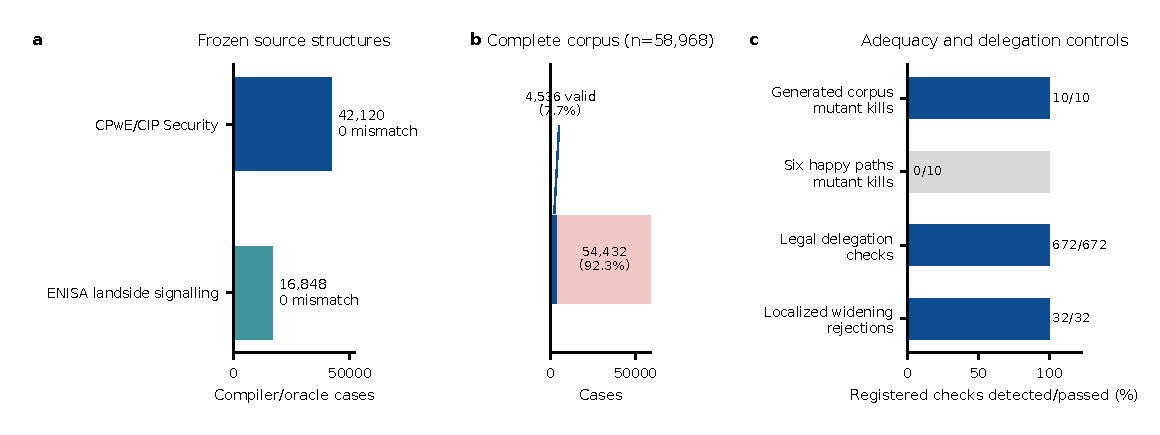
\includegraphics[width=\textwidth]{figures/generated/fig03_compiler_results}
\caption{Compiler agreement, corpus composition, and decisive controls. (a) Exact case counts from the two frozen source structures; the compiler and separate table oracle disagreed on none of them. (b) The complete 58,968-case corpus contains every 4,536 valid source-plus-overlay combination and 54,432 single-field mutations. (c) The generated corpus killed all 10 check-removal mutants, whereas six handwritten happy paths killed none; all 672 legal delegation-dimension checks passed and all 32 localized widening attempts were rejected. These seedless counts validate the frozen encoding and implementation checks, not the shared human interpretation of the source tables.}
\label{fig:compiler-results}
\end{figure*}

\subsection{Five Runtime Effects Preserved the Bounded Actuation-Event Refinement}

The main runtime run evaluated all 58,968 frozen one-request cases and one five-step composed trace for each of the 4,536 valid cases. Every effect was reached. No registered authority, parent-realizability, trace-inclusion, stutter, effect-order, or bounded-deadlock violation occurred, and all five negative-control mutants were detected. These observations apply to the registered actuation-event semantics, in which no-output decisions do not advance the plant.

The exhaustive study enumerated 492,156 words and 492,030 transitions through horizon five over 126 scopes. It covered all 25 effect bigrams and all 125 trigrams without a registered violation or deadlock, and it killed all three sequence-triggered mutants. In contrast, one named path per scope covered only four bigrams and three trigrams and killed none of those mutants. Exhaustive enumeration therefore tested interaction orders missed by individually effect-complete paths; it does not imply unbounded or asynchronous progress.

Replacing \texttt{ATTENUATE}, \texttt{REWRITE}, and \texttt{DEFER} with no-output denial preserved zero registered safety violations but removed behavior the frozen semantics treated as recoverable or safely corrected. Deny-only blocked 13,608 rewrite steps, or 16.67\% of the 81,648 constructed policy steps and 60\% of the constructed safe-service opportunities, and removed 9,072 attenuation or deferral recovery decisions. These fractions characterize the generated corpus, not an industrial workload distribution. Fig.~\ref{fig:runtime-results} separates effect incidence, interaction-order coverage, and physical-output loss.

\begin{figure*}[t]
\centering
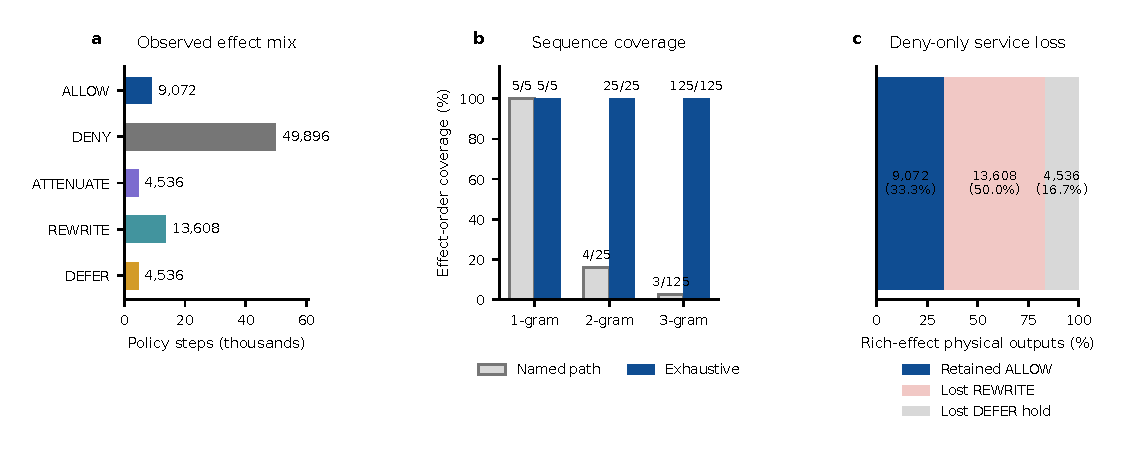
\includegraphics[width=\textwidth]{figures/generated/fig04_runtime_results}
\caption{Runtime-effect incidence, sequence coverage, and deny-only service loss. (a) Counts of the five observed effects over all 81,648 registered policy steps. (b) One named path per scope covered all five effects individually but only 4 of 25 effect bigrams and 3 of 125 trigrams; exhaustive enumeration through horizon five covered all 25 bigrams and 125 trigrams and killed all three sequence mutants, versus none for the named paths. (c) Of 27,216 physical outputs under the rich semantics, deny-only retained 9,072 ordinary allows while losing 13,608 corrected rewrites and 4,536 registered defer holds; it also removed 9,072 attenuation or deferral recovery decisions. All values are seedless exact counts, so no sampling error bars apply. Panel~(c) percentages use the 27,216 rich-semantics physical outputs as denominator, unlike the all-step (16.67\%) and safe-opportunity (60\%) rates in the text; all percentages describe the constructed corpus rather than field prevalence.}
\label{fig:runtime-results}
\end{figure*}

\begin{table*}[t]
\caption{Request-time correspondence of runtime authorization effects. Exact denotes the same request-time operational role; partial denotes related behavior at another lifecycle stage or without the registered physical contract; --- denotes that no source-grounded analogue was located. This is a mechanism comparison, not a performance ranking. Not shown: Lanotte/Roop additionally proves monitored-system deadlock freedom, which \zonecap{} checks only within its bounded registered models.}
\label{tab:effect-mapping}
\centering
\footnotesize
\setlength{\tabcolsep}{7pt}
\begin{tabular}{@{}lccccc@{}}
\toprule
System/profile & Allow & Deny & Live attenuation & Runtime rewrite & Approval defer/hold \\
\midrule
\zonecap{} & Exact & Exact & Exact & Exact & Exact \\
Lanotte/Roop edit automata & Exact & Exact & --- & Exact & --- \\
Pinned SINT profile & Exact & Exact & Partial & --- & Partial \\
\bottomrule
\end{tabular}
\end{table*}

Table~\ref{tab:effect-mapping} shows the source-grounded mechanism correspondence. Lanotte/Roop maps pass, suppress, and correction to three of the five effects, but has no mapped capability-attenuation or approval-stutter analogue. Pinned SINT maps allow and deny exactly, provides partial delegation-time attenuation and approval escalation, and has no runtime rewrite: all 13,608 registered \zonecap{} rewrites project to denial in the pinned profile. This mapping isolates lifecycle and effect roles. It neither subsumes the formal guarantees of prior enforcers nor compares their implementation scale.

% Conditional hardware subsection and Figure 6:
% Insert only after exp-22--25 pass the frozen audit. Report all five repetitions,
% worst-repetition p99, derived 10 ms scan occupancy (p99/10 ms, not an
% independent measurement), throughput, RSS, decision mismatch,
% ablations, scaling, and same-target executable baselines. If any repetition
% misses the registered threshold, report the refutation without seed selection.

\section{Revocation Boundary and Discussion}
\label{sec:discussion}

\subsection{Revocation Freshness: A Negative Result}

The initial concurrency model treated revocation delivery as an atomic resolver-local event. Through bound five, 793,800 event words produced 26,038 executions, 4,534 conflict resolutions, and 1,590 approval timeouts without a delivered-state revocation, permission-union, deterministic-order, or deadlock violation. Exact graph closure for two, three, and four holders converged at depths six, eight, and ten, reaching 1,110 states in total, including 461 states beyond bound five and 10,576 cycle edges, without exposing a new registered violation. These observations established only a local post-delivery boundary.

Separating issuance at the authority service from resolver delivery refuted the preregistered revocation claim, whose registered interpretation is issuance-relative. Each of five fixed scenarios used fair schedules with delay zero, one, or two, and every schedule eventually delivered the revocation. Delay zero produced no stale execution. Delays one and two each produced four, for eight issuance-relative stale executions in total, while all post-delivery and other registered checks remained clean. Fig.~\ref{fig:revocation} shows the resulting window. The counterexamples meet the preregistered false criterion and are not scheduler-nontermination artifacts.

\begin{figure}[t]
\centering
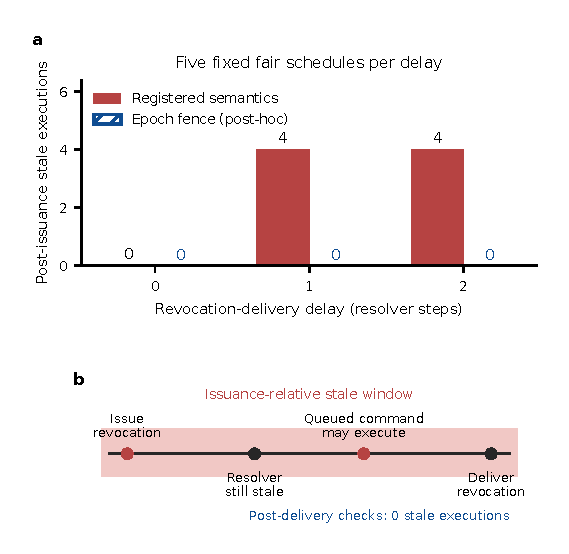
\includegraphics[width=\columnwidth]{figures/generated/fig05_revocation}
\caption{Delayed delivery refutes issuance-relative revocation safety. (a) Each delivery delay contains five fixed fair schedules. The registered semantics produced 0, 4, and 4 post-issuance stale executions at delays 0, 1, and 2, respectively; a post-hoc epoch-fence replay blocked all eight and is shown only as a diagnostic. (b) Revocation issuance opens a stale resolver window in which a queued command may execute before delivery. Every schedule eventually delivered revocation, and no post-delivery stale execution occurred.}
\label{fig:revocation}
\end{figure}

Pinned SINT exhibited the same boundary: before delivery it allowed one stale use and approved one already-queued revoked request, and only a fresh gateway recheck denied execution. An issuer-side epoch fence blocked all eight stale executions in a diagnostic replay. Neither the fence nor the gateway recheck repairs the registered \zonecap{} claim: the fence was introduced after the counterexample, and the SINT check belongs to a separate integration path. They instead identify the missing contract. A local resolver cannot establish issuance-relative safety unless execution is coupled to atomic delivery, a trusted freshness epoch, or a mandatory fresh execution-side check.

\subsection{Implications and Limitations}

The main result is an authorization-refinement interface rather than an intrinsic property of capability syntax. A compiler must establish authorization inclusion, and the runtime layer must establish request-abstracted emission inclusion through sound, parent-realizable outputs. This interface complements capability systems that provide identity, delegation, and cryptographic transport~\cite{dodson2021,dodson2020,sint2026,bamil2026} and runtime enforcers that provide correction, monitor synthesis, and scalable mediation~\cite{pearce2020,lanotte2023,baird2024}. It does not replace controller safety analysis or inherit guarantees that those systems did not claim.

The compiler evidence is intentionally bounded. The compiler and oracle use separate code paths, but both consume a single human-authored interpretation of each source. Provenance probes and mutants reduce shared implementation-error risk, not shared interpretation error. The five behavioral and contextual fields are a source-independent overlay, target assets are deterministic per-zone identifiers, and the ENISA input is a landside-signalling subgraph. The agreement therefore supports the frozen representation and delegation checks; it does not establish completeness for arbitrary IEC~62443 architectures or certification.

The runtime evidence is bounded to actuation events and horizon-five compositions. Real PLC scans advance when no new command is emitted, so fixed-tick integration must define the held output, controller memory, timeout, and plant evolution before re-establishing parent realizability. The current theorem also trusts the physical history, mode, and common plant relation. Compromised sensors, stale context, model mismatch, and asynchronous distributed effects require separate contracts. Finally, the theorem is manually written rather than machine checked, and the baseline projections compare expressible dimensions rather than complete deployed products.

No accepted target-hardware performance evidence is available at the current freeze. The local x86 run validated timer resolution, CPU affinity, forced-slow detection, and six disabled-check controls, but it did not measure the target Jetson Orin NX/OpenPLC path. It cannot support a latency, scan-occupancy, throughput, or memory claim. If the planned target-hardware study later passes its frozen raw-data and equivalence audits, it can be reported as prototype feasibility evidence; until then, the paper makes no performance claim.

\section{Conclusion}
\label{sec:conclusion}

\zonecap{} connects delegated industrial authorization to physical behavior through an explicit compiler-to-enforcer contract. Positive conjunctive attenuation establishes authorization inclusion, authorized and parent-realizable runtime effects establish request-abstracted emission inclusion, and a common plant relation lifts that result to finite-horizon trace and reachable-set inclusion. Exact enumeration, mutation controls, source-derived compiler tests, and bounded effect compositions challenged the concrete realization without substituting empirical scale for the conditional proof. The revocation counterexample further shows that local enforcement invariants do not establish issuance-relative safety without a freshness or atomic-delivery contract. The reusable result is therefore a set of inspectable obligations for physically refining industrial capabilities, bounded by trusted context, common plant semantics, actuation-event execution, and explicit revocation delivery.


\section*{Data and Code Availability}

The anonymized research artifact will provide the frozen source snapshots, policy tables, protocols, implementation, run configurations, commands, all registered seeds, logs, metrics, retained raw samples, and hash manifests used in this paper. \textbf{[AUTHOR INPUT NEEDED: insert a stable anonymous repository or archive URL before submission.]}


\begin{thebibliography}{99}

\bibitem{iec62443}
International Electrotechnical Commission, \emph{Security for Industrial Automation and Control Systems---Part 3-2: Security Risk Assessment for System Design}, IEC 62443-3-2:2020, 2020.

\bibitem{dodson2021}
M.~G. Dodson, ``Capability-based access control for cyber physical systems,'' Univ. Cambridge Computer Lab., Cambridge, U.K., Tech. Rep. UCAM-CL-TR-963, Oct. 2021.

\bibitem{dodson2020}
M. Dodson, A.~R. Beresford, A. Richardson, J. Clarke, and R.~N.~M. Watson, ``CHERI Macaroons: Efficient, host-based access control for cyber-physical systems,'' in \emph{Proc. IEEE Eur. Symp. Security Privacy Workshops}, 2020, pp. 688--693, doi: 10.1109/EuroSPW51379.2020.00099.

\bibitem{sint2026}
SINT Protocol, ``A layered open standard for security, governance, and economic enforcement in physical AI systems,'' white paper, ver. 0.2.0, Apr. 2026; implementation at commit 2461a911b8c3d7ed9da3f7662b33678f688eb826. [Online]. Available: \url{https://github.com/sint-ai/sint-protocol/tree/2461a911b8c3d7ed9da3f7662b33678f688eb826}

\bibitem{ranathunga2026}
T. Ranathunga, K. Fernando, and S. Rea, ``When agents control robots: A zero trust policy model for agentic cyber-physical systems,'' arXiv:2605.25653, 2026.

\bibitem{bamil2026}
V. Bamil, ``Delegation-aware runtime contracts for open LLM multi-agent systems: Constraint preservation, capability revocation, and state recovery,'' Research Square, preprint, 2026, doi: 10.21203/rs.3.rs-10533072/v1.

\bibitem{etigowni2016}
S. Etigowni, D.~J. Tian, G. Hernandez, S. Zonouz, and K. Butler, ``CPAC: Securing critical infrastructure with cyber-physical access control,'' in \emph{Proc. 32nd Annu. Conf. Computer Security Applications}, 2016, pp. 139--152, doi: 10.1145/2991079.2991126.

\bibitem{rafy2026}
M.~F. Rafy, ``TwinGridShield: Consequence-aware runtime authorization for LLM grid-agent actions,'' SSRN, preprint, 2026, doi: 10.2139/ssrn.7290820.

\bibitem{ligatti2005}
J. Ligatti, L. Bauer, and D. Walker, ``Edit automata: Enforcement mechanisms for run-time security policies,'' \emph{Int. J. Inf. Security}, vol. 4, nos. 1--2, pp. 2--16, Feb. 2005, doi: 10.1007/s10207-004-0046-8.

\bibitem{pearce2020}
H. Pearce, S. Pinisetty, P.~S. Roop, M.~M.~Y. Kuo, and A. Ukil, ``Smart I/O modules for mitigating cyber-physical attacks on industrial control systems,'' \emph{IEEE Trans. Ind. Informat.}, vol. 16, no. 7, pp. 4659--4669, Jul. 2020, doi: 10.1109/TII.2019.2945520.

\bibitem{lanotte2023}
R. Lanotte, M. Merro, and A. Munteanu, ``Industrial control systems security via runtime enforcement,'' \emph{ACM Trans. Privacy Security}, vol. 26, no. 1, Art. no. 4, Feb. 2023, doi: 10.1145/3546579.

\bibitem{baird2024}
A. Baird, A. Panda, H. Pearce, S. Pinisetty, and P. Roop, ``Scalable security enforcement for cyber physical systems,'' \emph{IEEE Access}, vol. 12, pp. 14385--14410, 2024, doi: 10.1109/ACCESS.2024.3357714.

\bibitem{schneider2000}
F.~B. Schneider, ``Enforceable security policies,'' \emph{ACM Trans. Inf. Syst. Security}, vol. 3, no. 1, pp. 30--50, Feb. 2000, doi: 10.1145/353323.353382.

\bibitem{dasilva2025}
M. Da~Silva, S. Mocanu, M. Puys, and P.-H. Thevenon, ``Safety-security convergence: Automation of IEC 62443-3-2,'' \emph{Comput. Security}, vol. 156, Art. no. 104477, Sep. 2025, doi: 10.1016/j.cose.2025.104477.

\bibitem{vaudey2024}
J. Vaudey, S. Mocanu, G. Delaval, and E. Rutten, ``An IEC 62443-security oriented domain specific modelling language,'' in \emph{Proc. 19th Int. Conf. Availability, Reliability Security}, 2024, pp. 1--10, doi: 10.1145/3664476.3670938.

\bibitem{cpwe2020}
Rockwell Automation, Cisco Systems, and Panduit, \emph{Deploying CIP Security Within a Converged Plantwide Ethernet Architecture}, Design Guide ENET-TD022A-EN-P, May 2020.

\bibitem{enisa2022}
European Union Agency for Cybersecurity, \emph{Zoning and Conduits for Railways}. Athens, Greece: ENISA, Feb. 2022, doi: 10.2824/761090.

\end{thebibliography}


\end{document}
